\documentclass[12pt, a4paper, spanish]{article}
\usepackage[spanish]{babel}
\usepackage[utf8]{inputenc}
\usepackage{setspace}
\usepackage[
pdftex,
pdfauthor={--- Arturo Vidal Peña ---},
pdftitle={--- Práctica 2 de Prolog ---},
hidelinks]{hyperref}

\usepackage{amssymb}
\usepackage{amsmath}
\usepackage{txfonts}
\usepackage{mathdots}

\usepackage{multicol}

% --- IMAGES ---
\usepackage{graphicx}
\usepackage{float}
\usepackage{subfigure}
\DeclareGraphicsExtensions{.png,.jpg,.pdf,.mps,.gif,.bmp}
% --- IMAGES ---

% --- MARGIN DIMENSIONS ---
\frenchspacing \addtolength{\hoffset}{-1.5cm}
\addtolength{\textwidth}{3cm} \addtolength{\voffset}{-2.5cm}
\addtolength{\textheight}{4cm}
\setlength{\headheight}{15pt}
% --- MARGIN DIMENSIONS ---

% --- CODE ---

\usepackage{listings}
\usepackage[usenames,dvipsnames]{color}

\definecolor{codegreen}{rgb}{0,0.6,0}
\definecolor{codegray}{rgb}{0.5,0.5,0.5}
\definecolor{codepurple}{rgb}{0.58,0,0.82}
\definecolor{backcolour}{rgb}{0.95,0.95,0.92}
\definecolor{predicate}{RGB}{250,202,43}


\lstdefinelanguage{Ciao-Prolog}{
	%keyword3
	classoffset = 2,
	morekeywords = {A, B, Comp, M, X, Y, Term1, Aridad1, Term2, Aridad2, Orden, ListaX, ListaY, Lista, Hojas, T, T1, T2, H, Arg1, Brg1, Arbol, Hoja, Tree,
		RaizIzq, Raiz, OrdenF, OrdenS, Element, Left, ElementRight, ListaSalida, Right},
	keywordstyle = \color{codegreen},	
	classoffset = 3,
	morekeywords = {arg, functor, call, var, nonvar, append},
	keywordstyle = \color{blue},	
	classoffset = 0,
	sensitive = true,
	morecomment = [l]{\%},
	morecomment = [s]{/*}{*/},
	commentstyle = \color{gray},
	morestring = [b]",
	morestring = [b]',
	stringstyle = \color{purple}
}
\lstset{
	language={Ciao-Prolog},
	basicstyle={\small},
	identifierstyle={\small},
	commentstyle={\small\itshape},
	keywordstyle={\small\bfseries},
	ndkeywordstyle={\small},
	stringstyle={\small\ttfamily},
	frame={tb},
	breaklines=true,
	columns=[l]{fullflexible},
	numbers=left,
	xrightmargin=0em,
	xleftmargin=3em,
	numberstyle={\scriptsize},
	stepnumber=1,
	numbersep=1em,
	lineskip=-0.5ex,
}


\lstdefinestyle{mystyle}{
	backgroundcolor=\color{backcolour},   
	commentstyle=\color{codegreen},
	keywordstyle=\color{blue},
	numberstyle=\tiny\color{codegray},
	stringstyle=\color{codepurple},
	basicstyle=\footnotesize,
	breakatwhitespace=false,         
	breaklines=true,                 
	captionpos=b,                    
	keepspaces=true,                 
	numbers=left,                    
	numbersep=5pt,                  
	showspaces=false,                
	showstringspaces=false,
	showtabs=false,                  
	tabsize=2
}

\lstset{style=mystyle}

% --- CODE ---

% --- TOC DOTS ---
\usepackage{tocloft}
\renewcommand{\cftsecleader}{\cftdotfill{\cftdotsep}}
% --- TOC DOTS ---

% --- TITLE DATA ---
\title{\textbf{Práctica 2: Programación en Prolog} \\
	\textsc{Programación Declarativa: Lógica y Restricciones} \\
	\emph{DIA}}
\author{\emph{Vidal Peña, Arturo}\\
		\emph{W140307}}
\date{\underline{\today}}
% --- TITLE DATA ---

\begin{document}
	
% --- TITLE ---
\maketitle
\thispagestyle{empty}
\pagenumbering{gobble}
\renewcommand*\contentsname{Índice de contenidos}
\tableofcontents
\pagebreak
% --- TITLE ---

\pagenumbering{arabic}

\section{Código empleado y las explicaciones}

\subsection{Predicado menor/4}
\lstinputlisting[language=Ciao-Prolog]{codeFiles/menor.pl}

En este predicado, preparo con \emph{functor/3} una estructura en \emph{X} de tres términos, y añado \emph{Comp, A} y \emph{B} con los predicados arg/3.\\

Luego, con \emph{call/1} llamo a esa estructura y guardo el resultado en \emph{M}.

\subsection{Predicado menor\_o\_igual/2}
 \lstinputlisting[language=Ciao-Prolog]{codeFiles/menor_o_igual.pl}

Para empezar, compruebo el primer caso de que alguna (o ambas) variables sean variables libres (\textit{menor\_o\_igual\_libre}).\\

En caso contrario (si ninguna de las dos lo es), extraigo de ambas variables su término y su aridad para contrastarlos. Este predicado se validará si se cumple alguno de los siguientes.

\subsubsection{Predicado menor\_o\_igual\_libre/2}
\lstinputlisting[language=Ciao-Prolog]{codeFiles/menor_o_igual_libre.pl}

Será cierto si alguno de los términos es una variable libre, igualándolo al otro. Si ninguno de los dos es una variable libre, volveríamos a \textit{menor\_o\_igual/2} para comprobar el resto de opciones.

\subsubsection{Predicado menor\_nombre/2}
\lstinputlisting[language=Ciao-Prolog]{codeFiles/menor_nombre.pl}

Este predicado, pasándole dos términos, se valida si el primero es menor que el segundo. Si no se validara, volvería a \textit{menor\_o\_igual/2}, donde se comprobaría el predicado \textit{menor\_aridad/4}.

\subsubsection{Predicado menor\_aridad/4}
\lstinputlisting[language=Ciao-Prolog]{codeFiles/menor_aridad.pl}

Este, recibe ambos términos y sus respectivas aridades y, comprobando que ambos términos son iguales, comprueba si la aridad del primero es menor a la del segundo. En el caso de que sea así, se valida. Si no, vuelve a \textit{menor\_o\_igual/2}, y pasa al predicado \textit{menor\_igual\_argumento/6}.

\subsubsection{Predicado menor\_o\_igual\_argumento/2}
\lstinputlisting[language=Ciao-Prolog]{codeFiles/menor_o_igual_argumento.pl}

Aquí, comprobamos primero que ambos términos son iguales, y que tienen la misma aridad. Luego, generamos en \textit{X} e \textit{Y} dos listas con sus respectivos términos y argumentos, para luego llamar a \textit{menor\_o\_igual\_argumento\_rec/2}.

\subsubsection{Predicado menor\_o\_igual\_argumento\_rec/2}
\lstinputlisting[language=Ciao-Prolog]{codeFiles/menor_o_igual_argumento_rec.pl}

Primero ponemos el caso base, con dos listas vacías de argumentos, que siempre será cierto.\\

En otro caso, comprobamos si los primeros argumentos de ambas listas pasadas son números, y comprobamos si el argumento de la primera lista es menor o igual al correspondiente en la segunda. Si no son números, hacemos la misma comprobación a nivel de término.\\

Hacemos esta llamada recursivamente, recorriendo ambas listas hasta que las acabamos (lista vacía), o encontramos un argumento en la primera lista que sea mayor al correspondiente en la segunda.

\subsection{Predicado lista\_hojas/2}
\lstinputlisting[language=Ciao-Prolog]{codeFiles/lista_hojas.pl}

Para este predicado, su caso base será con dos listas vacías.\\

En otro caso, recibiendo una lista de datos, genera una lista de hojas (o nodos) de la forma \textit{tree('dato', void, void)}, donde \textit{'dato'} es cada uno de los datos de la lista. Se llama recursivamente hasta acabar con todos los datos de la lista.

\newpage
\subsection{Predicado hojas\_arbol/3}
\lstinputlisting[language=Ciao-Prolog]{codeFiles/hojas_arbol.pl}

Este predicado llama a uno auxiliar recursivo \textit{hojasArbolRec/4}, con el primer dato de la lista de hojas como argumento extra.

\subsubsection{Predicado hojasArbolRec/3}
\lstinputlisting[language=Ciao-Prolog]{codeFiles/hojasArbolRec.pl}

El caso base consiste en una lista de hojas vacía, sin criterio de comparación, con el árbol como tercer y cuarto argumento. Básicamente, unifica el árbol de salida.\\

En otro caso, recibiendo una lista, extrae en \textit{RaizIzq} el dato de la hoja y en \textit{Raiz} la raíz actual del árbol, usando el predicado \textit{arg}. Luego, los compara extrayendo el menor según el criterio de comparación especificado en \textit{Comp} y guardándolo en \textit{M}; y por último, se llama de manera recursiva con el resto de la lista de hojas, el mismo criterio de comparación, un nuevo árbol con \textit{M} como raíz, el resto del árbol y el dato extraído de la lista de hojas; y el árbol de salida en el último argumento.\\

El árbol devuelto siempre tendrá nodos del tipo \textit{tree('dato',void,void)} en la parte derecha de cada nodo superior.

\subsection{Predicado ordenacion/3}
\lstinputlisting[language=Ciao-Prolog]{codeFiles/ordenacion.pl}

Este predicado, al igual que \textit{hojas\_arbol/3}, llama a uno auxiliar (\textit{ordenacion\_aux/4})con una lista vacía como argumento extra.

\subsubsection{Predicado ordenacion\_aux/4}
\lstinputlisting[language=Ciao-Prolog]{codeFiles/ordenacion_aux.pl}

Su caso base ocurre al tener sólo un nodo hoja en el árbol de entrada. El criterio de comparación por tanto no importa, ya que siempre será el último elemento a insertar (o el único). Por tanto, añade llamando a \textit{append/3} el dato del nodo al final de la lista \textit{Orden}, usando como parámetro de salida \textit{OrdenF}.\\

En otro caso, si hay más datos en el árbol, añade el primer  dato a una lista \textit{OrdenS}, luego crea una lista auxiliar \textit{Lista} con los elementos restantes llamando a \textit{makeList/3} y borra el elemento que acaba de insertar en \textit{OrdenS} de \textit{Lista}. Seguidamente crea un nuevo árbol a partir de \textit{Lista} llamando a \textit{lista\_hojas/2} y a \textit{hojas\_arbol/3}. Por último, se llama recursivamente con \textit{OrdenS} como nueva lista a la que añadir los elementos.

\subsubsection{Predicado makeList/3}
\lstinputlisting[language=Ciao-Prolog]{codeFiles/makeList.pl}

Su caso base se basa en un árbol de un único elemento y una lista cualquiera, devolviendo el elemento en la cabeza de la lista.\\

En otro caso, si hay varios elementos en el árbol, ignora el primer dato y extrae el elemento del nodo de la derecha, lo añade a una lista auxiliar \textit{Lista2} y se llama recursivamente con el resto del árbol (parte izquierda), \textit{Lista2} y la lista de salida en la que unificar en el caso base.

\subsubsection{Predicado borraElemento/3}
\lstinputlisting[language=Ciao-Prolog]{codeFiles/borraElemento.pl}

Este predicado tiene dos casos base:

\begin{itemize}
	\item Uno, en el que tiene que "borrar" un elemento de una lista vacía, en cuyo caso devuelve la misma lista vacía.
	
	\item Otro, en el que recibe un elemento que se encuentra en la cabeza de la lista, y devuelve la cola de la lista.
\end{itemize}

En otro caso (el elemento a borrar no se encuentra en la cabeza), se llama recursivamente con la cola de la lista, hasta que encuentre el elemento y lo elimine o ya no quede nada a borrar.

\subsection{Predicado ordenar/3}
\lstinputlisting[language=Ciao-Prolog]{codeFiles/ordenar.pl}

Este predicado llama a \textit{lista\_hojas/2}, \textit{hojas\_arbol/3} y \textit{ordenacion/3} con los argumentos que se le pasan.
\newpage

\section{Pruebas realizadas}
\subsection{menor/2}
\begin{multicols}{2}
	\begin{figure}[H]
		\centering
		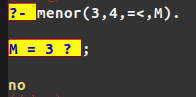
\includegraphics{images/menor1.png}
		\caption{3 $\leq$ 4}
	\end{figure}
	\begin{figure}[H]
		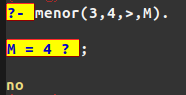
\includegraphics{images/menor2.png}
		\caption{3 $>$ 4}
	\end{figure}
\end{multicols}


\newpage
\section{Comentarios adicionales}

En mi opinión, considero que el enunciado de esta práctica no estaba correctamente redactado de manera que fuera de fácil comprensión. Considero que el haber necesitado dos ficheros de aclaraciones indica que hay algo a mejorar. Por otro lado, el enunciado de la primera práctica estaba mejor redactado y era más sencillo de comprender, con una explicación más clara de lo que se debía implementar y conseguir con cada predicado.\\

Ruego que se intente mejorar en la medida de lo posible para próximos años.
\end{document}

